% WISS collaborative photo booth system overview.
% Compile directly with pdfLaTeX in Overleaf (standalone document).
% For an article, copy the tikzpicture and load TikZ with the listed libraries.
\documentclass[tikz,border=8pt]{standalone}
\usepackage{tikz}
\usetikzlibrary{arrows.meta,backgrounds,fit,positioning}

\definecolor{clientblue}{HTML}{EAF3FB}
\definecolor{backendgray}{HTML}{F3F5F7}
\definecolor{datagreen}{HTML}{EAF5EE}
\definecolor{externalorange}{HTML}{FFF3E5}
\definecolor{wissblue}{HTML}{245A82}

\tikzset{
  flow/.style={-{Stealth[length=2.2mm]}, thick, draw=wissblue},
  bidiflow/.style={{Stealth[length=2.2mm]}-{Stealth[length=2.2mm]}, thick, draw=wissblue},
  notify/.style={-{Stealth[length=2.2mm]}, thick, dashed, draw=wissblue},
  client/.style={draw=wissblue, fill=clientblue, rounded corners=2pt,
    text width=3.35cm, minimum height=1.22cm, align=center, inner sep=5pt,
    font=\small},
  component/.style={draw=black!55, fill=white, rounded corners=2pt,
    text width=4.15cm, minimum height=0.76cm, align=center, inner sep=4pt,
    font=\small},
  backend/.style={draw=wissblue, fill=backendgray, rounded corners=4pt,
    inner sep=14pt, line width=1pt},
  store/.style={draw=black!55, fill=datagreen, rounded corners=2pt,
    text width=4.15cm, minimum height=1.02cm, align=center, inner sep=5pt,
    font=\small},
  external/.style={draw=black!55, fill=externalorange, rounded corners=2pt,
    text width=2.55cm, minimum height=0.9cm, align=center, inner sep=5pt,
    font=\small}
}

\begin{document}
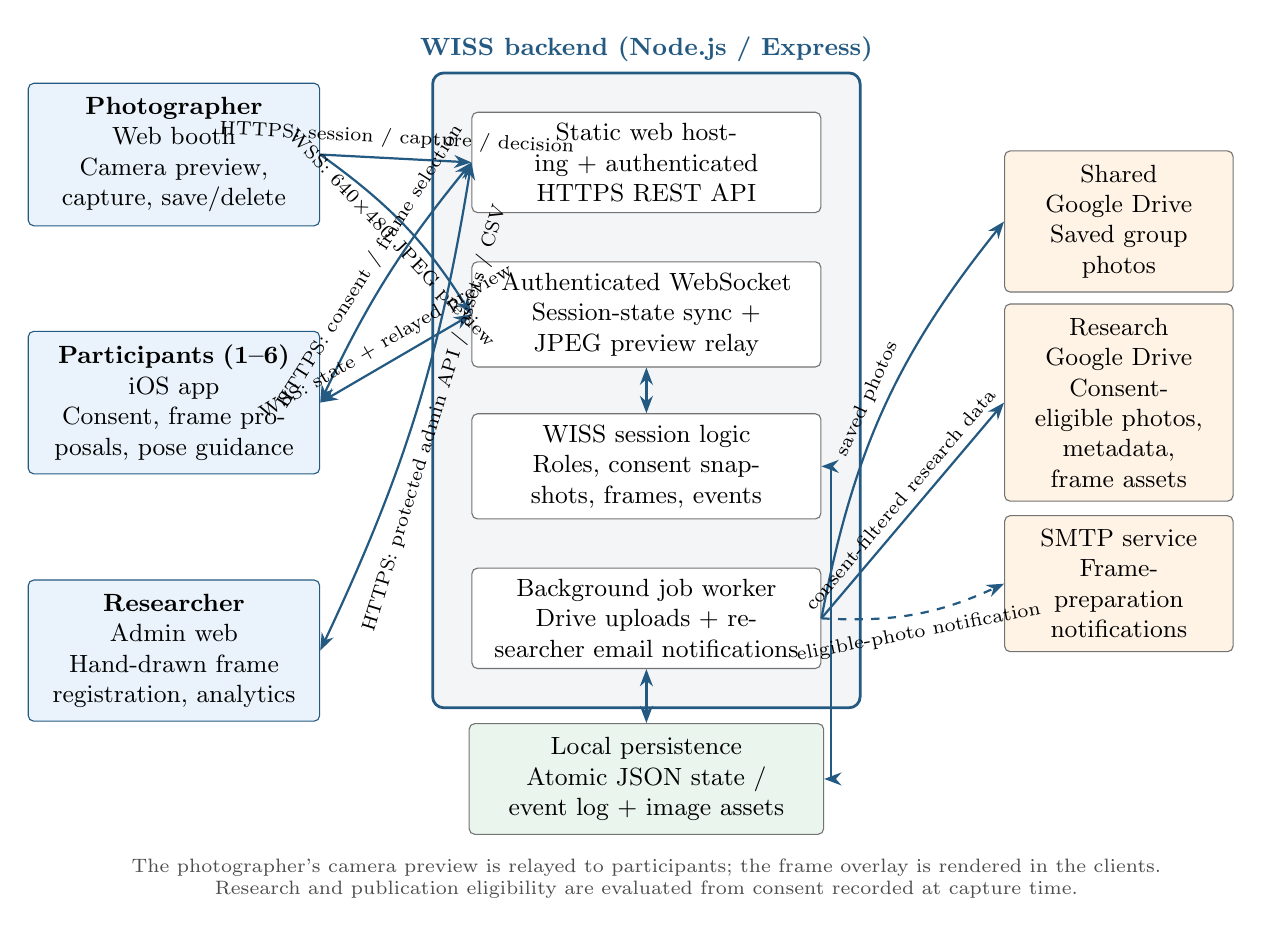
\begin{tikzpicture}[>=Stealth]
  % Human-facing clients
  \node[client] (photographer) at (0,3.15)
    {\textbf{Photographer}\\Web booth\\Camera preview, capture, save/delete};
  \node[client] (subjects) at (0,0)
    {\textbf{Participants (1--6)}\\iOS app\\Consent, frame proposals, pose guidance};
  \node[client] (researcher) at (0,-3.15)
    {\textbf{Researcher}\\Admin web\\Hand-drawn frame registration, analytics};

  % Backend modules
  \node[component] (api) at (6,3.05)
    {Static web hosting + authenticated HTTPS REST API};
  \node[component] (ws) at (6,1.12)
    {Authenticated WebSocket\\Session-state sync + JPEG preview relay};
  \node[component] (core) at (6,-0.81)
    {WISS session logic\\Roles, consent snapshots, frames, events};
  \node[component] (worker) at (6,-2.74)
    {Background job worker\\Drive uploads + researcher email notifications};

  \begin{scope}[on background layer]
    \node[backend, fit=(api)(ws)(core)(worker),
      label={[font=\bfseries\small, text=wissblue]above:WISS backend (Node.js / Express)}] (server) {};
  \end{scope}

  % Persistence and external services
  \node[store] (storage) at (6,-4.78)
    {Local persistence\\Atomic JSON state / event log + image assets};
  \node[external] (shared) at (12,2.3)
    {Shared Google Drive\\Saved group photos};
  \node[external] (researchdrive) at (12,0)
    {Research Google Drive\\Consent-eligible photos, metadata, frame assets};
  \node[external] (smtp) at (12,-2.3)
    {SMTP service\\Frame-preparation notifications};

  % Client-to-server communication
  \draw[flow] (photographer.east) -- node[above, sloped, font=\scriptsize, align=center]
    {HTTPS: session / capture / decision} (api.west);
  \draw[flow] (photographer.east) to[bend left=11]
    node[below, sloped, font=\scriptsize, align=center]
    {WSS: 640$\times$480 JPEG preview} (ws.west);

  \draw[bidiflow] (subjects.east) to[bend left=7]
    node[above, sloped, font=\scriptsize, align=center]
    {HTTPS: consent / frame selection} (api.west);
  \draw[bidiflow] (subjects.east) -- node[above, sloped, font=\scriptsize, align=center]
    {WSS: state + relayed preview} (ws.west);

  \draw[bidiflow] (researcher.east) to[bend right=8]
    node[below, sloped, font=\scriptsize, align=center]
    {HTTPS: protected admin API / assets / CSV} (api.west);

  % Internal services and persistence
  \draw[bidiflow] (ws.south) -- (core.north);
  \draw[bidiflow] (core.east) -- ++(0.12,0) |- (storage.east);
  \draw[bidiflow] (worker.south) -- (storage.north);

  % Asynchronous external integrations
  \draw[flow] (worker.east) to[bend left=14]
    node[above, sloped, font=\scriptsize, align=center]
    {saved photos} (shared.west);
  \draw[flow] (worker.east) -- node[above, sloped, font=\scriptsize, align=center]
    {consent-filtered research data} (researchdrive.west);
  \draw[notify] (worker.east) to[bend right=14]
    node[below, sloped, font=\scriptsize, align=center]
    {eligible-photo notification} (smtp.west);

  \node[font=\scriptsize, align=center, text=black!70] at (6,-6.05)
    {The photographer's camera preview is relayed to participants; the frame overlay is rendered in the clients.\\
     Research and publication eligibility are evaluated from consent recorded at capture time.};
\end{tikzpicture}
\end{document}
